%%%%%%%%%%%%%%%%%%%%%%%%%%%%%%%%%%%%%%%%%%%%%%%%%%%%%%%%%%%%%%%%%%%%%
% Use the koma-script document style
%\documentclass{scrbook}
%\KOMAoptions{twoside=false} % disable two-side formatting for scrbook
% alternatively, for shorter essay, use the following
\documentclass{scrartcl}
%%%%%%%%%%%%%%%%%%%%%%%%%%%%%%%%%%%%%%%%%%%%%%%%%%%%%%%%%%%%%%%%%%%%%

%%%%%%%%%%%%%%%%%%%%%%%%%%%%%%%%%%%%%%%%%%%%%%%%%%%%%%%%%%%%%%%%%%%%%
% Useful packages
\usepackage{mathtools}
\usepackage{amssymb,bm,bbold}
\usepackage[colorlinks=true]{hyperref}
\usepackage{enumerate}

\usepackage{wrapfig}
\usepackage{tikz}

%=================================
% pre-defined theorem environments
\usepackage{amsthm}
\newtheorem{theorem}{Theorem}
\newtheorem{lemma}{Lemma}
\newtheorem{proposition}{Proposition}
\newtheorem{corollary}{Corollary}
\newtheorem{definition}{Definition}
\newtheorem*{remark}{Remark}
\newtheorem*{assumption}{Assumption}

\usepackage[framemethod=tikz]{mdframed}
\newmdtheoremenv[
skipabove=\baselineskip,
skipbelow=\baselineskip,
hidealllines=true,
innertopmargin=4pt,
linewidth=4pt,
linecolor=gray!40,
singleextra={
  \draw[line width=3pt,gray!50,line cap=rect] (O|-P) -- +(1cm,0pt);
  \draw[line width=3pt,gray!50,line cap=rect] (O|-P) -- +(0pt,-1cm);
  \draw[line width=3pt,gray!50,line cap=rect] (O-|P) -- +(-1cm,0pt);
  \draw[line width=3pt,gray!50,line cap=rect] (O-|P) -- +(0pt,1cm);
  },
firstextra={
  \draw[line width=3pt,gray!50,line cap=rect] (O|-P) -- +(1cm,0pt);
  \draw[line width=3pt,gray!50,line cap=rect] (O|-P) -- +(0pt,-1cm);
},
secondextra={
  \draw[line width=3pt,gray!50,line cap=rect] (O-|P) -- +(-1cm,0pt);
  \draw[line width=3pt,gray!50,line cap=rect] (O-|P) -- +(0pt,1cm);
}
]{problem}{Problem}

%=================================
% useful commands
\DeclareMathOperator*{\argmin}{arg\,min}
\DeclareMathOperator*{\argmax}{arg\,max}
\DeclareMathOperator*{\supp}{supp}
\DeclareMathOperator*{\minimize}{\mathsf{minimize}}

\def\vec#1{{\ensuremath{\bm{{#1}}}}}
\def\mat#1{\vec{#1}}

%=================================
% convenient notations
\newcommand{\XX}{\mathbb{X}}
\newcommand{\RR}{\mathbb{R}}
\newcommand{\EE}{\mathbb{E}}
\newcommand{\PP}{\mathbb{P}}

\newcommand{\sB}{\mathcal{B}}
\newcommand{\sK}{\mathcal{K}}
\newcommand{\sL}{\mathcal{L}}

\newcommand{\TODO}{\textbf{\textsf{TODO}}}

\usepackage{algpseudocode}
\usepackage{algorithm}

%%%%%%%%%%%%%%%%%%%%%%%%%%%%%%%%%%%%%%%%%%%%%%%%%%%%%%%%%%%%%%%%%%%%%
% Typography, change document font
%\usepackage[libertine,cmintegrals,cmbraces,vvarbb]{newtxmath}
%\usepackage[scaled=0.95]{inconsolata}
\usepackage{lmodern}
\usepackage{charter}
\usepackage[scaled=0.95]{inconsolata}

\title{Intuitions for Optimization}
\author{pluskid}

\begin{document}
\maketitle

\section{Projected Subgradient Descent for Lipschitz Functions}

\subsection{Problem Setup}

\begin{problem}
  Given $f:\RR^n\rightarrow\RR$, and $\sK\subset\RR^n$. Assume $\sK$ is compact and convex, included
  in a Euclidean ball of radius $R$:
  \begin{equation}
    \sK \subset \sB_2(0; R)
  \end{equation}
  and $f$ is convex and $L$-Lipschitz on $\sK$:
  \begin{equation}
    |f(x)-f(y)| \leq L\|x-y\|_2, \quad x,y\in\sK
  \end{equation}
  Find the minimizer of $f$ on $\sK$:
  \[
  \minimize_{x\in\sK} f(x)
  \]
  \label{prob:projected-subgradient-descent}
\end{problem}

\subsection{Algorithm and its Bounds}

\begin{algorithm}
  \caption{Projected Subgradient Descent}
  \begin{algorithmic}
    \State randomly initialize $x^0\in\sK$
    \For{$t\gets 0,\ldots,T-1$}
      \State $y^{t+1}\gets x^{t}-\eta_t g_t$, where $g_t\in\partial f(x^{t})$
      \State $x^{t+1}\gets \Pi_{\sK}(y^{t+1})$
    \EndFor
  \end{algorithmic}
  \label{alg:projected-subgradient-descent}
\end{algorithm}

\begin{theorem}
  Running Algorithm~\ref{alg:projected-subgradient-descent} on Problem~\ref
  {prob:projected-subgradient-descent} for $T$ iterations gives
  \begin{equation}
  \min_{0\leq\tau\leq T}f(x^\tau) - f(x^*) \leq \frac{R^2 + G^2\sum_{t=0}^{T-1}\eta_t^2}{\sum_{t=0}^
  {T-1}\eta_t}
  \label{eq:proj-subgrad-bound}
  \end{equation}
  In general, the optimal bound is around $O(GR/\sqrt{T})$ with stepsizes around $\eta_t\eqsim R/
  (G\sqrt{t})$. That means in order to get an approximate error of $\varepsilon$, we will need to
  run the algorithm for $O(1/\varepsilon^2)$ iterations.
  \label{thm:projected-subgradient-descent}
\end{theorem}

\subsection{Intuitions and Analysis}

\subsubsection{Problem Assumptions}
\label{sec:subgrad-descent-assumption}

We consider the unconstrained case first, i.e. $\sK=\RR^n$. Since $f$ is convex know that $x^*$ is a
minimizer of $f$ if and only if $0\in\partial f (x^*)$. However, without making any extra
assumptions, we have no idea of the behavior of $f$ even in a small neighborhood of $x^*$. Consider
for example $f(x)=C|x|$, with $C>0$ a large constant. Assume we are currently very close to the
optimal $x^*=0$, say $x^t=\varepsilon$, $\varepsilon>0$. $f$ is differentiable at $\varepsilon$, so
the only subgradient is $g_t=C$. Therefore,
\[
  x^{t+1} = x^t - \eta_t g_t
  = \varepsilon - \eta_tC < -\varepsilon, \quad \forall \eta_t > \frac {2\varepsilon} {C}
\]
As we can see, unless the stepsize $\eta_t$ is very tiny, we will overshoot, $f(x^{t+1})>f(x^t)$.
Moreover, if we use a constant stepsize $\eta_t=\eta$, then if $\eta >\varepsilon/C$, we will be
jumping back and forth at $\varepsilon$ and $\varepsilon - \eta C$ indefinitely.

In order to fix this, we need to make additional assumptions. We will see later in the case of
smooth functions, the gradient changes continuously. So we know that at a local neighborhood of the
optimal (gradient is 0), the gradient is also small. But here, we are working with
non-differentiable functions, we will just assume $f$ is $L$-Lipschitz.

Note $f$ being $L$-Lipschitz in $\sK$ implies that $\|g\|_2 \leq L$, $\forall g\in\partial f(x),
\forall x\in\sK$. In order to avoid overshooting, we will have to move with tiny stepsizes.

\subsubsection{Convergence Analysis}

By the property of subgradient, we have
\begin{equation}
  0\leq f(x^t) - f(x^*) \leq g_t^\top (x^t-x^*) = -g_t^\top (x^*-x^t)
\end{equation}
\begin{wrapfigure}{r}{.4\linewidth}
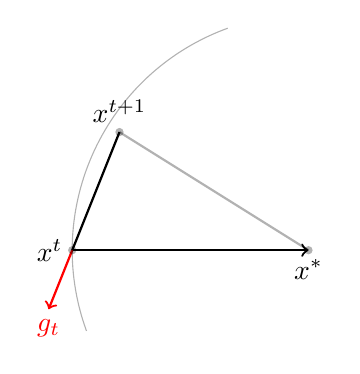
\begin{tikzpicture}[scale=1.5]
  \coordinate [label=left:$x^t$] (Xt) at (-2,0);
  \coordinate [label=below:$x^*$] (Xs) at (0,0);
  \coordinate [label=above:$x^{t+1}$] (Xtp) at (-1.6,1);
  \draw [->,thick] (Xt) -- (Xs);
  \draw [thick] (Xt) -- (Xtp);
  \draw [thick,opacity=.3] (Xs) -- (Xtp);
  \draw [->,thick,red] (Xt) -- (-2.2,-0.5) node [below] {$g_t$};

  \fill [black,opacity=.3] (Xt) circle (1pt);
  \fill [black,opacity=.3] (Xtp) circle (1pt);
  \fill [black,opacity=.3] (Xs) circle (1pt);
  \draw [opacity=.3] ([shift=(110:2)] 0,0) arc (110:200:2);
\end{tikzpicture}
\caption{Demonstration of subgradient descent.}
\label{fig:subgrad-descent-demo}
\end{wrapfigure}
where the left hand side is due to the optimality of $x^*$. This inequality indicates that the
vector $x^*-x^t$ is non-negatively correlated with $-g_t$, the direction of a subgradient descent.

Unlike in the case of differentiable functions, in which we can guarantee that the function values
decreases when moving along the direction of negative gradient with a small enough step size; here
we do not know much about the function values. But as we can see from Figure~\ref
{fig:subgrad-descent-demo}, when the angle between $-g_t$ and $x^*-x^t$ is greater than or equal to $\pi/2$,
we will move away from $x^*$ with any positive step size. However, if $f(x^t)-f(x^*)>0$, i.e. we are
not already at the optimal, the angle is strictly less than $\pi/2$, so if we move with a small
enough step size, we will get closer to $x^*$. Algebraically,
\[
\begin{aligned}
  \|x^{t+1}-x^*\|^2 = \|x^{t+1}-x^t + x^t-x^*\|^2
  &= \eta_t^2\|g_t\|^2 + \|x^t-x^*\|^2 - 2\eta_tg_t^\top (x^t-x^*) \\
  &\leq {\color{red}\eta_t^2\|g_t\|^2} + \|x^t-x^*\|^2 - {\color{blue}2\eta_t\left(f(x^t)-f
  (x^*)\right)} \\
\end{aligned}
\]
Since $\|g_t\|\leq L$ by our assumption, the \textcolor{red}{red term} decays quadratically, while
the \textcolor{blue}{blue term} only decays linearly. So when $\eta_t$ is small enough, we will have
$\|x^{t+1}-x^*\|^2 \leq \|x^t-x^*\|^2$. Furthermore, the progress we make by moving towards $x^*$ is
characterized by $f(x^t)-f(x^*)$. So if we are still far away from the optimal, we will be making
quite a lot progress in each step. On the other hand, when $f(x^t)-f(x^*)$ is small, our progress
might be small, but at that point we are already close to the optimal function value $f(x^*)$.

Actually, to get a bound on the algorithm, we can just sum up the previous inequality for all
$t=0,\ldots,T-1$,
\[
  \begin{aligned}
    0\leq\|x^T-x^*\|^2
    &\leq \|x^0-x^*\|^2 + \sum_{t=0}^{T-1}\eta_t^2\|g_t\|^2 - 2\sum_{t=0}^{T-1}\eta_t \left(f(x^t)-f
    (x^*)\right) \\
    &\leq R^2 + G^2\sum_{t=0}^{T-1}\eta_t^2 -2\left(\min_{0\leq\tau\leq T}f(x^\tau) - f
    (x^*)\right)\sum_{t=0}^{T-1}\eta_t
  \end{aligned}
\]
It then implies
\begin{equation}
\min_{0\leq\tau\leq T}f(x^\tau) - f(x^*) \leq \frac{R^2 + G^2\sum_{t=0}^{T-1}\eta_t^2}{\sum_{t=0}^
{T-1}\eta_t}
\end{equation}
which proved Theorem~\ref{thm:projected-subgradient-descent} for the case of unconstrained
optimization ($\sK=\RR^n$).

\subsection{Choosing Stepsizes}

Note \eqref{eq:proj-subgrad-bound} holds for any choices of stepsizes $\eta_t$ (though some of them
will give completely trivial bounds). So we could actually optimize the right hand side to get an
``optimal'' bound. To make the problem easier, we choose a fixed stepsize $\eta_t=\eta$ for
$t=0,\ldots,T-1$. So the right hand side becomes
\begin{equation}
  \frac{R^2+G^2T\eta^2}{T\eta} = \frac{R^2}{T\eta} + G^2\eta \geq \frac{2GR}{\sqrt{T}}
  \label{eq:subgrad-bound-fix-eta}
\end{equation}
where the inequality holds with equality when
\begin{equation}
  \eta = \frac{R}{G\sqrt{T}}
\end{equation}
Note the choice of step size depends on several factors:
\begin{description}
  \item[$G$:] As we described in Section~\ref{sec:subgrad-descent-assumption}, large $G$ will force
  us to be careful and move with small stepsizes. Our intuition is consistent here.
  \item[$R$:] In our analysis, we only use $R$ to bound $\|x^0-x^*\|$. When $R$ is large, we want to
  use large step size, otherwise we might never reach the optimal in the given time budget $T$.
  Generally when $x^*$ is unknown, $R$ can be bounded by the size of $\sK$ for the case
  of constrained optimization.
  \item[$T$:] The inverse dependency on $T$ can be interpreted as: when having a large time budget,
  we can be a little bit more careful and move slowly.
\end{description}


However, in general, the fact that the stepsize depends on the total number of iterations is
strange. That means if I want to compute more iterations, I will have to start over again and use a
different stepsize if I want to bound the performance with formula.

In general, we will prefer to use a decaying learning rate. Specifically, as long as
$\sum_t\eta_t\rightarrow \infty$ and $\sum_t\eta_t^2$ is bounded or approaches infinity at a slower
rate than $\sum_t\eta_t$, \eqref{eq:proj-subgrad-bound} will give a reasonable bound. For example,
take $\eta_t=R/(G\sqrt{t+1})$, since
\[
\begin{aligned}
  \sum_{t=0}^{T-1} \frac{1}{t+1} &\leq 1 + \int_1^{T} \frac{1}{x}\,dx = 1 + \log T \\
  \sum_{t=0}^{T-1} \frac{1}{\sqrt{t+1}} &\geq \int_1^{T+1}\frac{1} {\sqrt{x}}\,dx =
  2\sqrt{T+1}-2
\end{aligned}
\]
Plug-in to \eqref{eq:proj-subgrad-bound}, we get
\begin{equation}
  \min_{0\leq \tau \leq T} f(x^\tau) - f(x^*) \leq GR \frac{1+\log T}{2\sqrt{T+1}-2} \lesssim \frac
  {GR\log T}{\sqrt{T}}
\end{equation}
Comparing with the optimal bound we get with a fixed stepsize in \eqref{eq:subgrad-bound-fix-eta},
we lose a factor of $\log T$, but our stepsize does not depend on the total number of iterations any
more.

\subsubsection{Constrained Optimization}


%\bibliographystyle{alpha}
%\bibliography{bibfile}

\end{document}
